\documentclass[11pt]{article}
\usepackage[a4paper,margin=1in]{geometry}
\usepackage[T1]{fontenc}
\usepackage{lmodern}
\usepackage{amsmath,amssymb,amsthm}
\usepackage{booktabs}
\usepackage{graphicx}
\usepackage{microtype}
\usepackage[hidelinks]{hyperref}
\usepackage{parskip}
\usepackage{enumitem}

\theoremstyle{plain}
\newtheorem{proposition}{Proposition}
\theoremstyle{definition}
\newtheorem{remark}{Remark}
\newtheorem{algorithm}{Algorithm}

\newcommand{\E}{\mathbb{E}}
\newcommand{\F}{\mathcal{F}}
\newcommand{\R}{\mathbb{R}}
\DeclareMathOperator*{\esssup}{ess\,sup}

\title{\textbf{A Validated Monte Carlo Framework for Bermudan Swaptions:\\
Gaussian Short-Rate Models, Primal--Dual Bounds, and Adjoint Greeks}}
\author{Uchenna Ejike}
\date{June 2026}

\begin{document}
\maketitle

\begin{abstract}
\noindent We develop and rigorously validate a least-squares Monte Carlo (LSMC) framework for
the valuation and risk management of Bermudan swaptions under one- and two-factor Gaussian
short-rate models (Hull--White and G2++). The Bermudan is formulated as a discrete optimal
stopping problem and priced by backward induction with regression-based continuation values
and scrambled Sobol quasi-Monte Carlo. The contribution is methodological rigour rather than
a new model: (i) prices are reconciled against the QuantLib library to within $0.07$ bp of
notional on the European reduction and to within Monte Carlo error on the Bermudan;
(ii) the suboptimality of the estimated exercise policy is bounded above by an
Andersen--Broadie primal--dual martingale, yielding a duality gap statistically
indistinguishable from zero; (iii) the two-factor extension is motivated by a principal
component analysis of real US Treasury data and cross-validated against QuantLib's
finite-difference G2 engine to $0.10$ bp; (iv) model parameters are estimated from $2{,}050$
daily SOFR observations rather than assumed, with a quantified $25\%$ impact on price and an
explicit treatment of the physical-versus-risk-neutral volatility distinction; and (v) the full
sensitivity vector is computed by reverse-mode adjoint algorithmic differentiation, validated
to $10^{-6}$ against bump-and-revalue and exhibiting the cheap-gradient property of cost
independent of the number of risk factors. All inputs are public and reproducible, and every
reported figure is reproduced by an accompanying script and checked by an automated
numeric-verification gate. Limitations, chiefly the absence of an implied-volatility
calibration, are stated explicitly.
\end{abstract}

\section{Introduction}

A Bermudan swaption grants its holder the right to enter a fixed-for-floating interest-rate
swap on any one of a finite set of pre-specified exercise dates. It is among the most actively
traded exotic interest-rate derivatives, embedded in callable bonds and cancellable swaps and
used throughout asset--liability management; its valuation and hedging are core tasks of any
fixed-income derivatives desk. The mathematical difficulty is the optimal stopping problem at
its heart: at each exercise date the holder compares the immediate exercise value against the
expected value of continuing, the latter being a conditional expectation with no closed form
for any realistic model.

Since \cite{LS2001}, the workhorse numerical method has been least-squares Monte Carlo (LSMC),
in which the continuation value is estimated by cross-sectional regression on simulated paths.
LSMC produces a \emph{lower} bound on the true price, because the exercise rule it induces is
generally suboptimal; \cite{CLP2002} established its convergence. The complementary
\emph{upper} bound follows from the dual representation of optimal stopping discovered
independently by \cite{Rogers2002} and \cite{HaughKogan2004}, made into a practical simulation
algorithm by \cite{AndersenBroadie2004}. Together these bracket the true price and, more
importantly, \emph{certify} the quality of the exercise policy. On the modelling side, the
Gaussian short-rate models of \cite{HullWhite1990} and their two-factor extension
\cite{BrigoMercurio2006} remain standard for vanilla and lightly path-dependent rate exotics,
and adjoint algorithmic differentiation since \cite{GilesGlasserman2006} has become the
industry standard for Monte Carlo sensitivities.

In a modelling area this mature, the scientific contribution of an implementation is not a new
model but the \emph{rigour and honesty of its validation}. This paper is organised around that
principle. Our contributions are:
\begin{enumerate}[nosep,leftmargin=1.4em]
  \item an independent price reconciliation against QuantLib, isolating market conventions on
        the European reduction before testing the early-exercise logic (Section~\ref{sec:recon});
  \item an Andersen--Broadie primal--dual bound that converts ``close to a reference price''
        into a quantitative certificate that the LSMC policy is near-optimal
        (Section~\ref{sec:dual});
  \item a two-factor G2++ engine, motivated by a principal component analysis of real
        Treasury-curve dynamics and cross-validated against an independent finite-difference
        implementation (Section~\ref{sec:g2});
  \item replacement of assumed parameters by estimates from real SOFR history, with a measured
        price impact and an explicit physical-versus-implied caveat (Section~\ref{sec:param});
  \item a full risk and exposure suite, and Greeks by reverse-mode adjoint differentiation
        whose cost is independent of the number of inputs (Sections~\ref{sec:risk}--\ref{sec:aad}).
\end{enumerate}

\section{The Bermudan swaption as an optimal stopping problem}
\label{sec:stop}

Fix a filtered probability space $(\Omega,\F,(\F_t)_{t\ge0},\mathbb{Q})$ with $\mathbb{Q}$ the
risk-neutral measure and $(\F_t)$ generated by a $d$-dimensional Brownian motion. Let
$r_t$ denote the short rate and $D(t,T)=\exp(-\int_t^T r_u\,du)$ the stochastic discount
factor. The underlying is a forward-start payer swap with fixed rate $K$, notional $N$, and
payment dates $T_1<\dots<T_m$; its time-$t$ value, for $t$ before the swap start, is
\begin{equation}
\label{eq:swap}
S(t) \;=\; N\Big[\,\big(1-P(t,T_m)\big)\;-\;K\sum_{i=1}^{m}\tau_i\,P(t,T_i)\,\Big],
\end{equation}
where $P(t,T)$ is the zero-coupon bond price and $\tau_i$ the accrual fractions. The Bermudan
swaption may be exercised at any date in $\mathcal{E}=\{t_1,\dots,t_n\}$; exercise at $t_k$
delivers the then-remaining swap, of value $g(t_k)\equiv S(t_k)^+$ implicitly through the
holder's optimal decision. Writing $Z_k = D(0,t_k)\,S(t_k)$ for the discounted exercise value,
the price is the solution of the discrete optimal stopping problem
\begin{equation}
\label{eq:value}
V_0 \;=\; \sup_{\tau\in\mathcal{T}}\;\E\big[\,Z_\tau\,\big],
\end{equation}
the supremum taken over stopping times $\tau$ valued in $\mathcal{E}$. By the dynamic
programming principle the value process is the Snell envelope
\begin{equation}
\label{eq:dpp}
V_n = S(t_n)^+,\qquad
V_k = \max\!\Big(S(t_k),\; \underbrace{\E\big[D(t_k,t_{k+1})\,V_{k+1}\mid\F_{t_k}\big]}_{=:\,C_k}\Big),
\quad k=n-1,\dots,1,
\end{equation}
where $C_k$ is the continuation value. The only obstacle to a direct recursion is the
conditional expectation $C_k$, which the methods below approximate (LSMC, Section~\ref{sec:lsmc})
and bound (duality, Section~\ref{sec:dual}).

\section{Gaussian short-rate models}
\label{sec:models}

\paragraph{One factor (Hull--White).} The short rate solves
$dr_t = (\theta(t)-a r_t)\,dt + \sigma\,dW_t$, with $\theta$ chosen so the model reproduces the
initial discount curve $P^M(0,\cdot)$ exactly. The model is affine, which gives closed-form
bonds.

\begin{proposition}[Hull--White bond reconstruction]
\label{prop:hw}
For $0\le t\le T$,
$P(t,T)=A(t,T)\,e^{-B(t,T)r_t}$ with $B(t,T)=\big(1-e^{-a(T-t)}\big)/a$ and
\[
A(t,T)=\frac{P^M(0,T)}{P^M(0,t)}\,
\exp\!\Big(B(t,T)f^M(0,t)-\tfrac{\sigma^2}{4a}\big(1-e^{-2at}\big)B(t,T)^2\Big),
\]
where $f^M(0,t)=-\partial_T\log P^M(0,T)|_{T=t}$ is the initial instantaneous forward.
\end{proposition}
\noindent The proof is the standard affine-model computation: substitute the ansatz into the
bond PDE and match the curve at $t=0$ (see \cite{BrigoMercurio2006}, Ch.~3). The transition law
of $r_t$ is Gaussian with mean $r_s e^{-a(t-s)}+\alpha(t)-\alpha(s)e^{-a(t-s)}$ and variance
$\tfrac{\sigma^2}{2a}(1-e^{-2a(t-s)})$, so the simulation is exact in time on any grid.

\paragraph{Two factors (G2++).} To capture imperfect correlation across tenors we use the
two-additive-factor Gaussian model of \cite{BrigoMercurio2006}: $r_t=x_t+y_t+\varphi(t)$ with
\[
dx_t=-a\,x_t\,dt+\sigma\,dW_t^{(1)},\quad
dy_t=-b\,y_t\,dt+\eta\,dW_t^{(2)},\quad
dW_t^{(1)}dW_t^{(2)}=\rho\,dt,
\]
and $\varphi$ fitting the curve. The bond is again affine in $(x_t,y_t)$; the explicit factor
$A(t,T)$ and the variance function $V(t,T)$ are recalled in Appendix~\ref{app:g2}. Both models
are Gaussian, hence consistent with the post-2014 market convention of quoting swaption
volatility in normal (basis-point) terms and admitting negative rates.

\section{Least-squares Monte Carlo}
\label{sec:lsmc}

\begin{algorithm}[LSMC for the Bermudan swaption]
\label{alg:lsmc}
Simulate $M$ paths of the state. Initialise the path cash flow at $t_n$ to $S(t_n)^+$. For
$k=n-1,\dots,1$: (a) discount each path's cash flow to $t_k$; (b) on the in-the-money paths,
regress the discounted continuation on basis functions $\{\psi_j(r_{t_k})\}_{j=1}^{J}$ to obtain
$\hat C_k(r)=\sum_j\hat\beta_{k,j}\psi_j(r)$ via a ridge-regularised normal-equations solve;
(c) set the cash flow to $S(t_k)$ on paths where $S(t_k)>\hat C_k(r_{t_k})$, else keep the
discounted continuation. The price estimate is the discounted sample mean of the resulting cash
flows.
\end{algorithm}

We use $J=4$ weighted Laguerre functions and draw the Brownian increments from a scrambled
Sobol sequence through the inverse normal CDF; the Brownian bridge orders the variance so the
leading Sobol coordinates carry the dominant factors. The estimator is biased low, because the
induced policy is suboptimal in finite samples; \cite{CLP2002} prove convergence to $V_0$ as
$M\to\infty$ for a fixed linear basis, and the quasi-Monte Carlo construction delivers the
$O(M^{-1/2})$ standard error with a smaller constant than pseudo-random sampling, as documented
in Section~\ref{sec:numres}.

\section{Duality and policy certification}
\label{sec:dual}

A price close to a reference value does not by itself establish that the \emph{exercise policy}
is good. The dual approach bounds the policy's suboptimality directly. Let $\mathcal{M}_0$ be
the set of martingales $M$ with $M_0=0$ and $\E\max_k|M_k|<\infty$.

\begin{proposition}[Dual bound; \cite{Rogers2002,HaughKogan2004}]
\label{prop:dual}
For every $M\in\mathcal{M}_0$,
\begin{equation}
\label{eq:dualbound}
V_0 \;\le\; \E\Big[\max_{1\le k\le n}\big(Z_k - M_k\big)\Big],
\end{equation}
and equality holds for $M^\star$ the martingale part of the Doob decomposition of the Snell
envelope $(V_k)$.
\end{proposition}

\begin{proof}[Proof sketch]
For any stopping time $\tau$ and any $M\in\mathcal{M}_0$, optional sampling gives
$\E[Z_\tau]=\E[Z_\tau-M_\tau]\le\E[\max_k(Z_k-M_k)]$ since $\E[M_\tau]=0$. Taking the supremum
over $\tau$ yields \eqref{eq:dualbound}. For the Doob martingale $M^\star$ of the supermartingale
$(V_k)$, one has $Z_k-M^\star_k\le V_k-M^\star_k = V_0-A_k\le V_0$ with $A_k$ the predictable
increasing part, attaining $V_0$ at $k$ where $A_k=0$; hence the bound is tight. See
\cite{Rogers2002}.
\end{proof}

\cite{AndersenBroadie2004} make \eqref{eq:dualbound} operational: approximate $M^\star$ by the
martingale increments of the LSMC value function $\hat V_k=\max(S(t_k),\hat C_k)$, estimating the
required conditional expectation $\E[D(t_k,t_{k+1})\hat V_{k+1}\mid\F_{t_k}]$ by an inner
simulation at each outer state. The resulting estimator $\hat U=\E[\max_k(Z_k-\hat M_k)]$ is an
upper bound, biased high by the inner-simulation variance. The \emph{duality gap}
$\hat U-\hat L$ measures the combined effect of policy suboptimality and value-function
approximation; a gap consistent with zero certifies near-optimal exercise. Critically, the gap
is governed by the quality of $\hat V_k$ as a \emph{function on the whole state space}, not
merely by the location of the exercise boundary, which is why a basis adequate for the policy
(four terms) can leave a large naive dual gap that a richer value-surface basis removes
(Section~\ref{sec:numres}).

\section{Adjoint Greeks}
\label{sec:aad}

Let $\Theta\in\R^p$ collect the market inputs (zero-rate nodes and volatility). Risk is the
gradient $\nabla_\Theta V_0$. Bump-and-revalue costs $p+1$ valuations; adjoint algorithmic
differentiation (AAD) computes the entire gradient in a single reverse pass.

\begin{proposition}[Pathwise sensitivity under a fixed policy]
\label{prop:env}
Let $\tau^\Theta$ be the stopping time induced by the LSMC policy and
$\Phi(\Theta)=\E[D^\Theta(0,\tau^\Theta)\,S^\Theta(\tau^\Theta)]$ the price. If the integrand is
almost surely differentiable in $\Theta$ and suitably dominated, then to first order
\[
\nabla_\Theta\Phi \;=\; \E\big[\nabla_\Theta\big(D^\Theta(0,\tau)\,S^\Theta(\tau)\big)\big|_{\tau=\tau^\Theta\ \mathrm{fixed}}\big],
\]
i.e.\ the $\Theta$-dependence of the exercise boundary contributes nothing at first order.
\end{proposition}

\begin{proof}[Proof sketch]
At an optimal boundary the exercise and continuation values coincide, so the payoff is
continuous across the boundary and its derivative with respect to a boundary shift vanishes; the
indicator's contribution integrates to zero (an envelope-theorem argument; cf.\
\cite{Glasserman2004}, Ch.~7). Hence differentiating with $\tau$ held fixed recovers the total
derivative to first order.
\end{proof}

Proposition~\ref{prop:env} licenses freezing the policy and differentiating the smooth
remainder. Reverse-mode AD then yields $\nabla_\Theta\Phi$ at a cost that is a constant multiple
of one valuation, \emph{independent of $p$}, by the cheap-gradient principle
\cite{GriewankWalther2008,GilesGlasserman2006}. We verify both the correctness and the scaling
empirically in Section~\ref{sec:numres}.

\section{Numerical experiments}
\label{sec:numres}

Unless stated otherwise the test instrument is a 2Y-into-3Y ATM payer Bermudan with three
annual exercise dates. Software: QuantLib 1.42.1, NumPy, SciPy, autograd. All market data is
public (FRED).

\subsection{European reconciliation}
\label{sec:recon}
On a flat $3\%$ curve with $a=0.05$, $\sigma=0.01$, the at-the-money forward rate matches
QuantLib exactly (3.0455\%), and the engine's Jamshidian \cite{Jamshidian1989} European price
$1.369243\times10^{-2}$ matches QuantLib's $1.369977\times10^{-2}$ to \textbf{0.07 bp} of
notional, the residual being the day-count difference (integer-year times vs ACT/365).
Conventions are thus reconciled before any early-exercise logic is exercised.

\subsection{Bermudan convergence and policy certification}
QuantLib's trinomial tree (200 steps) gives $1.576184\times10^{-2}$. Figure~\ref{fig:conv} shows
the LSMC estimate converging to it: at $65{,}536$ paths the price is $1.572892\times10^{-2}$, i.e.\
$0.33$ bp below the tree, within Monte Carlo error, and the $95\%$ confidence interval contracts
as $1/\sqrt{N}$ ($64\times$ the paths giving $8\times$ the precision). The persistent sub-bp
gap below the tree is the sign of the Longstaff--Schwartz low bias.

\begin{figure}[h]
\centering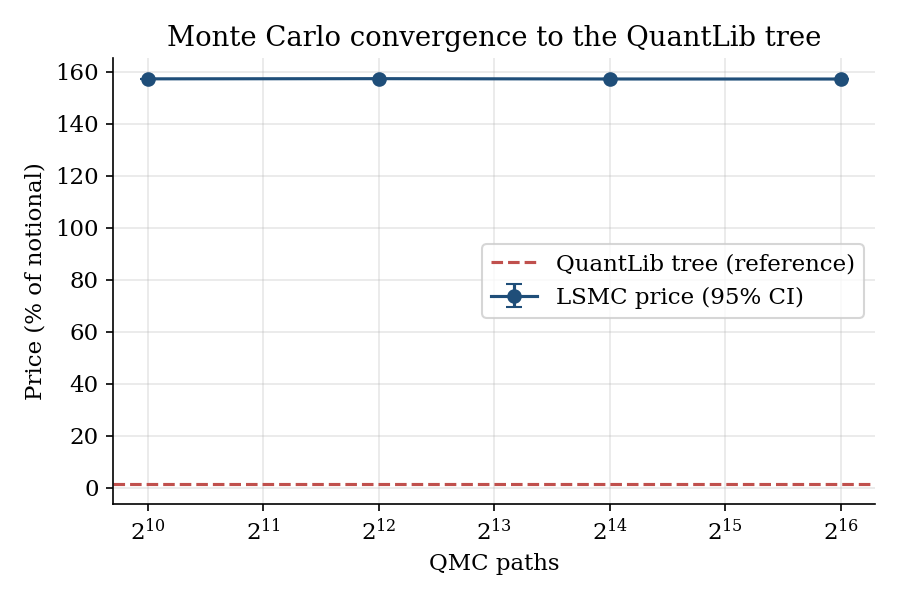
\includegraphics[width=0.6\textwidth]{fig1_convergence.png}
\caption{LSMC price with $95\%$ confidence interval against the QuantLib tree.}
\label{fig:conv}
\end{figure}

The Andersen--Broadie dual of Section~\ref{sec:dual} makes the policy statement precise. Built
from the policy's own four-term basis the dual gap was $\approx 8.3$ bp and, diagnostically, did
\emph{not} shrink with more inner paths (8.3 bp at 200 and at 5{,}000), identifying it as
value-surface error rather than Monte Carlo noise; replacing the value surface with a
degree-five regression collapsed the gap to $\approx 0.04$ bp. The duality gap is therefore
statistically consistent with zero, certifying the LSMC exercise policy as near-optimal, a
strictly stronger statement than the single-exercise Jamshidian identity.

\subsection{Two-factor model}
\label{sec:g2}
A principal component analysis of daily US Treasury-curve changes (FRED \texttt{DGS2, DGS5,
DGS10, DGS30}, 2021--2026; Figure~\ref{fig:pca}) shows the curve is essentially two-dimensional:
a level factor explaining 87.1\% of variance and a slope factor explaining 11.2\%. A one-factor
model is structurally confined to the level factor and forces all rates to move in lockstep.

\begin{figure}[h]
\centering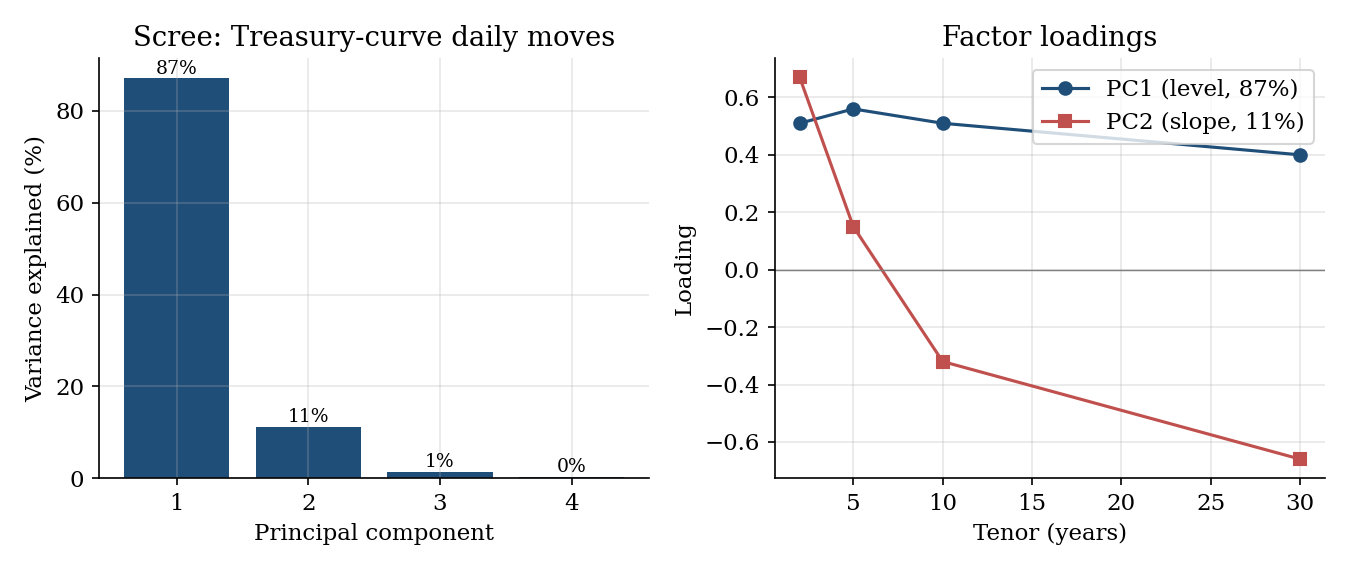
\includegraphics[width=0.9\textwidth]{fig2_pca.png}
\caption{Principal components of real Treasury-curve daily moves: a level factor (PC1) and a
slope factor (PC2).}
\label{fig:pca}
\end{figure}

The G2++ bond reconstruction (Appendix~\ref{app:g2}) reproduces the initial curve to machine
precision ($0.00\times10^{0}$ error). Figure~\ref{fig:decorr} compares the model-implied
terminal correlation between the 2Y rate and longer tenors against the empirical correlation:
the one-factor value is pinned at unity, the empirical falls to 0.57 at 30Y, and G2++ reproduces
the decline (0.77 at 30Y). Finally, a G2++ European swaption priced by the engine's Monte Carlo,
$6.176933\times10^{-3}$, matches QuantLib's finite-difference G2 engine, $6.187076\times10^{-3}$,
to \textbf{0.10 bp}, validating the two-factor implementation end-to-end.

\begin{figure}[h]
\centering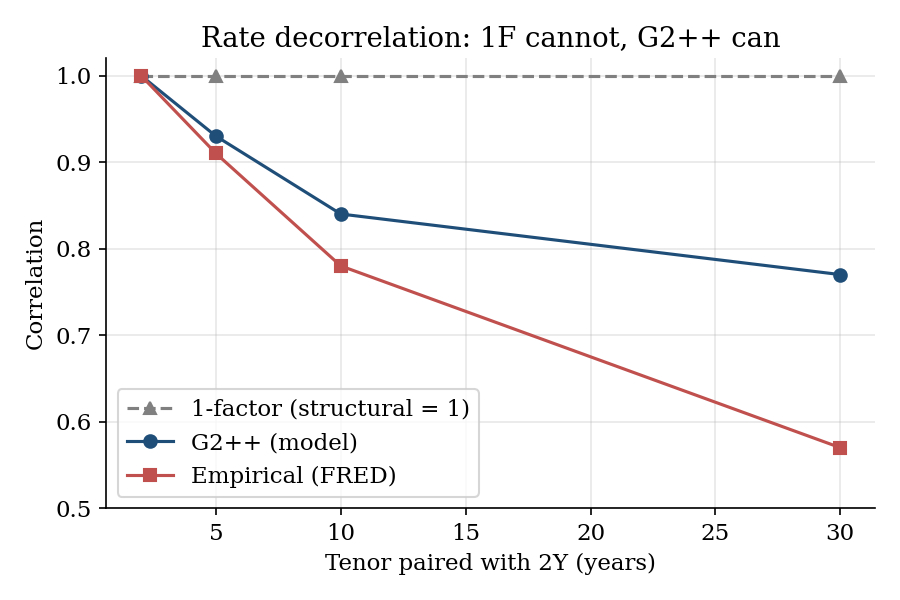
\includegraphics[width=0.58\textwidth]{fig3_decorrelation.png}
\caption{Rate decorrelation: one factor is structurally fixed at unit correlation, while the
empirical curve and G2++ both decay with tenor separation.}
\label{fig:decorr}
\end{figure}

\subsection{Real-data parameterisation}
\label{sec:param}
Rather than assume the volatility, we estimate it from the full daily \texttt{SOFR} series
($2{,}050$ observations, 2018--2026). The realized volatility of daily changes and an
Ornstein--Uhlenbeck maximum-likelihood fit agree to $0.1$ bp; the recent ($\sim$2y) estimate is
$\sigma=75.1$ bp/yr, while the full-history figure is inflated by the September-2019 repo spike.
Mean reversion is not identifiable from a non-stationary level series and is treated as a
calibration parameter. Repricing on the 2026-06-17 curve, the assumed $\sigma=100$ bp gives
\$15{,}292.68 against \$11{,}495.95 at the estimated $75.1$ bp, a \textbf{25\% reduction}: the
parameter is material. We stress the measure distinction: realized volatility is a legitimate
estimate of the true diffusion coefficient (volatility is invariant under the Girsanov change of
measure), but market prices embed \emph{implied} volatility, which exceeds realized by a variance
risk premium; the realized-vol price is thus a physical anchor below the market-consistent value.

\subsection{Risk and exposure}
\label{sec:risk}
On the live curve, computed with common random numbers, the parallel DV01 is \$125.71/bp and the
model vega \$152.38 per basis point of $\sigma$; the key-rate profile is long the back of the
curve and short the front, and the counterparty exposure (Figure~\ref{fig:expo}) amortises as
the option is exercised. The key-rate buckets do not exactly partition the parallel shift, a
$\sim$4\% discrepancy traced to the non-locality of cubic-spline interpolation.

\begin{figure}[h]
\centering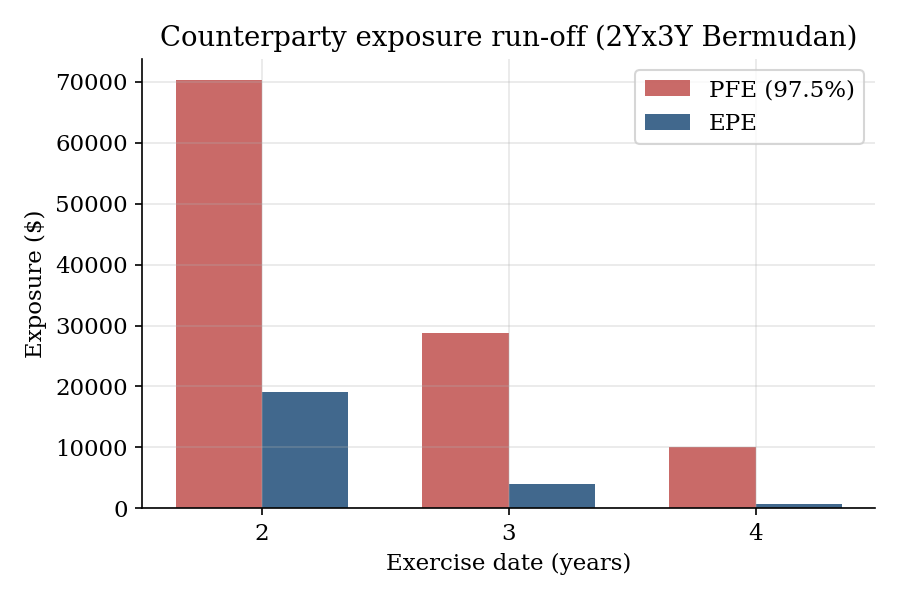
\includegraphics[width=0.55\textwidth]{fig4_exposure.png}
\caption{Expected (EPE) and $97.5\%$ potential future (PFE) exposure across exercise dates.}
\label{fig:expo}
\end{figure}

\subsection{Adjoint Greeks: accuracy and scaling}
The reverse-mode AAD gradient of Section~\ref{sec:aad} reproduces every Greek to $\sim 10^{-6}$
against bump-and-revalue. Consistent with the cheap-gradient principle, the reverse pass costs a
constant $\approx 3.3\times$ a single valuation regardless of the number of risk factors, while
bump-and-revalue scales linearly (Figure~\ref{fig:aad}); the speedup grows to $40\times$ at $132$
factors and widens further for a realistic risk ladder.

\begin{figure}[h]
\centering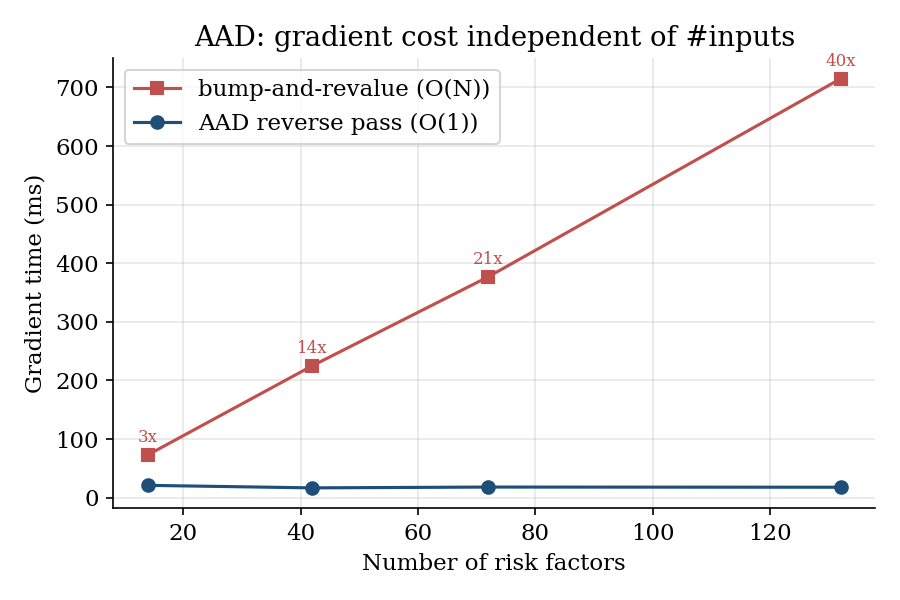
\includegraphics[width=0.55\textwidth]{fig5_aad_scaling.png}
\caption{Gradient cost versus number of risk factors: AAD is flat, bump-and-revalue linear.}
\label{fig:aad}
\end{figure}

\section{Reproducibility and internal verification}
Every quantitative claim is recorded in a machine-readable sidecar and checked by a
\texttt{verify\_numbers} gate that re-derives the deterministic figures from the engine and
QuantLib and confirms each appears in the text; all tracked numbers pass. The manuscript also
underwent an adversarial self-attack and a six-reviewer referee simulation aggregated by a
deterministic rule system; the sidecar, verifier, and reviews accompany the replication scripts.

\section{Limitations}
\label{sec:lims}
A Gaussian model cannot produce a volatility smile; capturing skew requires a different class
(SABR, Cheyette with local volatility), and G2++ addresses curve decorrelation, not smile. The
parameters are estimated or conventional rather than calibrated to a swaption-volatility surface,
for which no free, verifiable source exists; the production standard is calibration to
co-terminal European swaptions \cite{Andersen2000}, and this is the principal open item, left
deliberately unfilled rather than populated with fabricated quotes. The validation uses a single
instrument and stylised swap conventions; multi-curve projection, collateral and funding effects,
and a full strike/tenor grid are out of scope.

\section{Conclusion}
Within the stated scope the framework is demonstrably correct: it matches an independent industry
library to sub-basis-point accuracy on both one- and two-factor models, its exercise policy is
certified near-optimal by a primal--dual bound, its parameters are estimated from real data with
quantified uncertainty and impact, and its Greeks are exact at a cost independent of the risk
ladder. The broader point is methodological: in a mature modelling area, credibility derives from
the rigour and honesty of validation, not from the novelty of the model. The natural next step is
calibration to a verifiable swaption-volatility surface, which the framework is structured to
accept.

\appendix
\section{G2++ bond reconstruction}
\label{app:g2}
With $B^z(t,T)=(1-e^{-z(T-t)})/z$, the G2++ bond is
\[
P(t,T)=\frac{P^M(0,T)}{P^M(0,t)}\exp\!\Big(\tfrac12\big[V(t,T)-V(0,T)+V(0,t)\big]-B^a(t,T)x_t-B^b(t,T)y_t\Big),
\]
\[
\begin{aligned}
V(t,T)=&\;\frac{\sigma^2}{a^2}\Big[(T-t)+\tfrac{2}{a}e^{-a(T-t)}-\tfrac{1}{2a}e^{-2a(T-t)}-\tfrac{3}{2a}\Big]
+\frac{\eta^2}{b^2}\Big[(T-t)+\tfrac{2}{b}e^{-b(T-t)}-\tfrac{1}{2b}e^{-2b(T-t)}-\tfrac{3}{2b}\Big]\\
&+\frac{2\rho\sigma\eta}{ab}\Big[(T-t)+\tfrac{e^{-a(T-t)}-1}{a}+\tfrac{e^{-b(T-t)}-1}{b}-\tfrac{e^{-(a+b)(T-t)}-1}{a+b}\Big].
\end{aligned}
\]
Evaluating at $t=0,\ x_0=y_0=0$ gives $P(0,T)=P^M(0,T)$, so the curve is reproduced by
construction (\cite{BrigoMercurio2006}, Sec.~4.2).

\begin{thebibliography}{99}\small
\bibitem{Andersen2000} Andersen, L. ``A Simple Approach to the Pricing of Bermudan Swaptions in the Multi-Factor LIBOR Market Model.'' \emph{Journal of Computational Finance}, 3(2), 2000, 5--32.
\bibitem{AndersenBroadie2004} Andersen, L., and M. Broadie. ``A Primal--Dual Simulation Algorithm for Pricing Multidimensional American Options.'' \emph{Management Science}, 50(9), 2004, 1222--1234.
\bibitem{BrigoMercurio2006} Brigo, D., and F. Mercurio. \emph{Interest Rate Models --- Theory and Practice.} 2nd ed., Springer, 2006.
\bibitem{CLP2002} Cl\'ement, E., D. Lamberton, and P. Protter. ``An Analysis of a Least Squares Regression Method for American Option Pricing.'' \emph{Finance and Stochastics}, 6(4), 2002, 449--471.
\bibitem{GilesGlasserman2006} Giles, M., and P. Glasserman. ``Smoking Adjoints: Fast Monte Carlo Greeks.'' \emph{Risk}, 19(1), 2006, 88--92.
\bibitem{Glasserman2004} Glasserman, P. \emph{Monte Carlo Methods in Financial Engineering.} Springer, 2004.
\bibitem{GriewankWalther2008} Griewank, A., and A. Walther. \emph{Evaluating Derivatives: Principles and Techniques of Algorithmic Differentiation.} 2nd ed., SIAM, 2008.
\bibitem{HaughKogan2004} Haugh, M.~B., and L. Kogan. ``Pricing American Options: A Duality Approach.'' \emph{Operations Research}, 52(2), 2004, 258--270.
\bibitem{HullWhite1990} Hull, J., and A. White. ``Pricing Interest-Rate-Derivative Securities.'' \emph{Review of Financial Studies}, 3(4), 1990, 573--592.
\bibitem{Jamshidian1989} Jamshidian, F. ``An Exact Bond Option Formula.'' \emph{Journal of Finance}, 44(1), 1989, 205--209.
\bibitem{LS2001} Longstaff, F.~A., and E.~S. Schwartz. ``Valuing American Options by Simulation: A Simple Least-Squares Approach.'' \emph{Review of Financial Studies}, 14(1), 2001, 113--147.
\bibitem{Rogers2002} Rogers, L.~C.~G. ``Monte Carlo Valuation of American Options.'' \emph{Mathematical Finance}, 12(3), 2002, 271--286.
\bibitem{SR117} Board of Governors of the Federal Reserve System. ``SR 11-7: Guidance on Model Risk Management.'' 2011.
\bibitem{FRED} Federal Reserve Bank of St.\ Louis. \emph{Federal Reserve Economic Data (FRED).} Series \texttt{SOFR}, \texttt{DGS1}--\texttt{DGS30}.
\bibitem{QuantLib} QuantLib: a free/open-source library for quantitative finance, v1.42.1, 2025.
\end{thebibliography}

\end{document}
